\RequirePackage{fix-cm}
\documentclass[smallextended]{svjour3}       % onecolumn (second format)
\smartqed  % flush right qed marks, e.g. at end of proof
\usepackage{graphicx,multicol,lipsum,caption,authblk}
\usepackage{amsmath,booktabs,verbatimbox,tikz}
\usepackage[numbers,sort]{natbib}
\usepackage{geometry,pgf,pgfplots,}
\usepackage{mathptmx}
\usetikzlibrary{shapes.geometric, matrix,arrows,positioning,calc,intersections}
\usepackage{booktabs, makecell, multirow, threeparttable}
\usepackage{tablefootnote}
\usepackage{stackengine}
\begin{document}



\title{Laminated Composite Plate Optimization by Genetic Algorithm}
\titlerunning{Stacking Sequence Optimization}        % if too long for running head
\author{Zhang Huiyao$^1$  \and
	Atsushi Yokoyama $^{1,*}$
}
\authorrunning{Zhang Huiyao} % if too long for running head
\institute{Zhang Huiyao \at
              Room 203,Bulding 3,Kyoto Institue of Technology\\
			  Matsugasaki,Sakyo-ku,Kyoto,606-8585,JAPAN\\
              \email{zhanghy1012@gmail.com}           %  \\
           \and
           S. Author \at
              second address
}
\date{Received: date / Accepted: date}
\maketitle

\begin{abstract}
Failure analysis of laminated composite plates under different mechanical loads for different
stacking sequences, fiber orientation, and composite material system is studied in this paper.
An optimum composite material and laminate layup is studied for a targeted strength ratio which
makes a compromise between weight and cost through genetic algorithm.


\keywords{Genetic Algorithm \and Laminates \and Stacking Sequence \and Hybrid Composites}
\end{abstract}

%\begin{multicols}{2}
%\begin{multicols}


\section{Introduction}
% 第一段
% 第一句话,FRP复合材料在众多领域都有着广泛的应用,因为它具有很高的强度比等性质.
Composites material offer improved strength, stiffness, fatigue, and corrosion
resistance, etc over conventional materials, which is widely used in
automotive, aerospace, and ship building industry.  However, the high cost of
fabrication of composites is a critical drawback for its application, for
example, the graphite/epoxy composite part may cost as much as \$650 to \$900
per kilogram, while the price of glass/epoxy is about 2.5 times less.  The
mechanical performance of a composite is affected by a wide range of factors,
thickness, material,number and orientation of a lamina.

In typical engineering applications, composite materials are under very
complicate loading conditions, not only in-plane loads but also out-of-plane
loads. Most of the studies on the optimization of laminated composite materials
was to mimimize the thickness \cite{abu1998optimum,walker2003technique},
weight\cite{fang1993design,deka2005multiobjective,park2008improved}, cost and
weight\cite{deka2005multiobjective,omkar2008artificial}, or maximize the static
strength of composite laminates for a targeted
thickness\cite{walker2003technique,lin2004stacking,kim2007development}. In the
present study, laminate cost and weight are minimized by modifying the objective function.

To tailor a laminate composite, genetic algorithm(GA) has been successfully
applied to solve laminate design
problem\cite{riche1993optimization,nagendra1996improved,sadagopan1998application,todoroki1998stacking,liu2000permutation,sivakumar1998optimum,walker2003technique,lin2004stacking,kang2005minimum,murugan2007target,akbulut2008optimum}.
GA simulates the process of natural evolutionary includes selection, crossover, 
and mutation according to Darwin's principal of "survival of the fittest".
Selection is the most important operator  of GA which decides the diversity of
the population.  In this step, if the selection pressure increases, the
converge speed of the population increases, however, the diversity of the
population decrease.  To improve the search ability and reduce the search cost,
various selection methods has been invented, and the selection schemes can be
divided into four classes which are proportionate reproduction, ranking,
tournament, and genitor(or ”steady state”) selection. In the optimization of
laminated composite structure, roulette wheel\cite{riche1993optimization,seresta2007optimal} and
tournament\cite{lin2004stacking} have been applied.
The pros of GA as the following: (i): GAs are not easily trapped in local
optima, and be able to obtain the global optimal. (ii): GA doesn't need
gradient information and can be applied to discrete optimization problem.
(iii): GA not only be able to find the optimal value in the domain, but also
can maintain a set of optimal solutions


In order to check the feasibility of a composite laminate by imposing a
strength constraint, failure analysis of a laminate is taken by applying
suitable failure criteria. The previous researchers adopted the
first-ply-failure approach using the Tsai-wu failure theory
\cite{massard1984computer,reddy1987first,fang1993design,soeiro1994multilevel,pelletier2006multi,jadhav2007parametric,omkar2008artificial,choudhury2019failure},
Tsai-Hill\cite{martin1987optimum,soares1995discrete}, the maximum
stress\cite{jadhav2007parametric,omkar2008artificial}, or the maximum
strain\cite{watkins1987multicriteria} static failure criteria. In the present
study, Tsai-wu static failure criteria is used to investigated the feasibility
of a composite laminate.



\section{Stress and Strain in a Laminate}
A laminated structure is consisting of multiple laminas bonded together through
their thickness.  Consider a laminated composite plate which is symmetric to
its middle plane and subjected to in-plane loads of extension, shear, bending
and torsion,  the classical lamination theory(CLT) is taken to calculate the
stresses and strains in the local and global axes of each ply. as shown in
Fig.\ref{fig:lamina}.

\begin{center}
  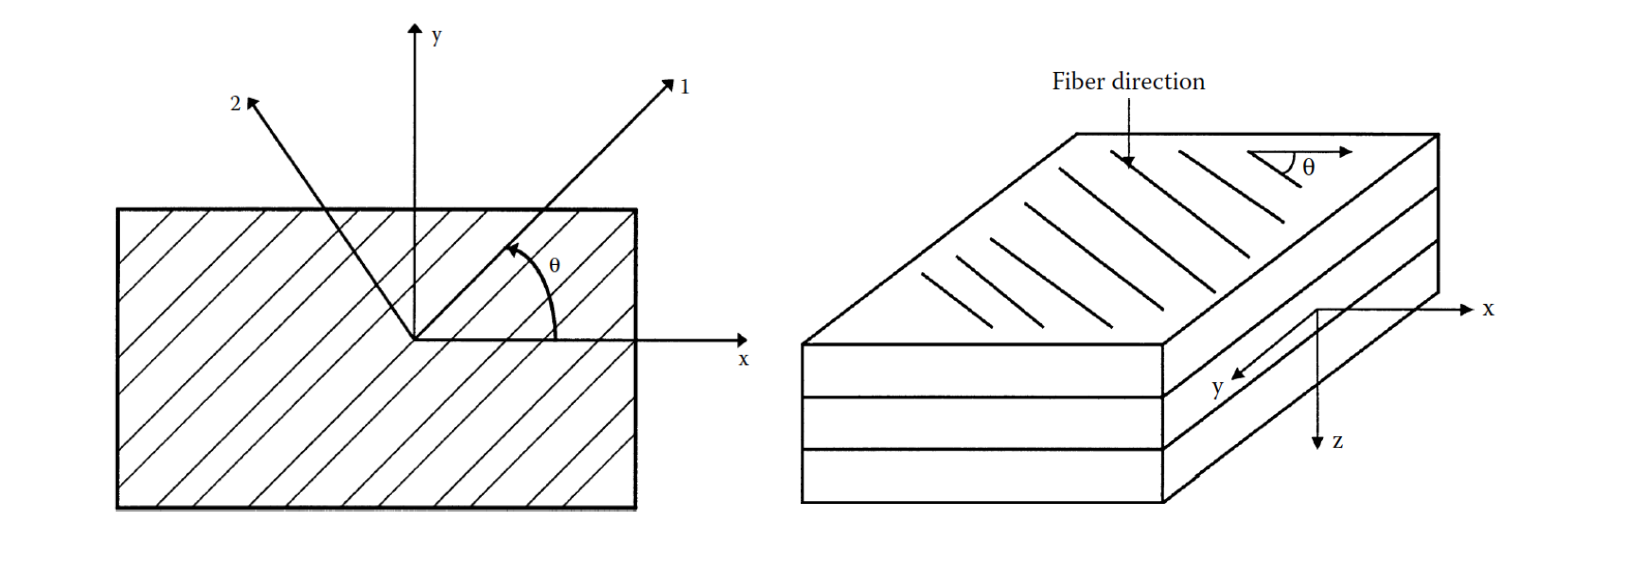
\includegraphics[width=\linewidth]{A_laminate_design_images/lamina_local_global_axes.png}
  \captionof{figure}{Lamina}
  \label{fig:lamina}
\end{center}

\subsection{Stress and Strian in a Lamina}
For a single lamina, the stress strain relation in the local axis.
\begin{equation}
    \begin{bmatrix}
        \sigma_1\\
        \sigma_2\\
        \tau_{12}
    \end{bmatrix}
    =
    \begin{bmatrix}
        Q_{11} & Q_{12} & 0\\
        Q_{12} & Q_{22} & 0\\
        0      &  0     & Q_{66}
    \end{bmatrix}
    \begin{bmatrix}
        \varepsilon_1\\
        \varepsilon_2\\
		\gamma_{12}
    \end{bmatrix}
\end{equation}
Where $Q_{ij}$ are the stiffnesses of the lamina that are related to 
engineering elastic constants by
\begin{equation}
    \begin{split}
    &Q_{11}=\frac{E_1}{1-v_{12}v_{21}}\\
    &Q_{22}=\frac{E_2}{1-v_{12}v_{21}}\\
    &Q_{66}=G_{12}\\
    &Q_{12}=\frac{v_{21}E_2}{1-v_{12}v_{21}}\\
    \end{split}
\end{equation}

Where, $E_1, E_2, v_{12}, G_{12}$ are four independent engineering elastic constants, they are
defined as 
\vspace{3mm}

$E_1$ = longitudinal Young's modulus(in direction 1)

$E_2$ = transverse  Young's modulus(in direction 1)

$v_{12}$ = major Poisson's ratio

$G_{12}$ = in-plane shear modulus (in plane 1-2)
\vspace{3mm}

Stress strain relation in global axis are

\begin{equation}
	\left[\begin{array}{l}\sigma_{x} \\ \sigma_{y} \\ \tau_{x
			y}\end{array}\right]=\left[\begin{array}{lll}\bar{Q}_{11} & \bar{Q}_{12} & \bar{Q}_{16}
			\\ \bar{Q}_{12} & \bar{Q}_{22} & \bar{Q}_{26} \\ \bar{Q}_{16} & \bar{Q}_{26} &
			\bar{Q}_{66}\end{array}\right]\left[\begin{array}{l}\varepsilon_{x} \\ \varepsilon_{y}
	\\ \gamma_{x y}\end{array}\right]
\end{equation}

where

\begin{equation}
	\begin{array}{l}
		\bar{Q}_{11}=Q_{11} c^{4}+Q_{22} s^{4}+2\left(Q_{12}+2 Q_{66}\right) s^{2} c^{2}
		\\ 
		\bar{Q}_{12}=\left(Q_{11}+Q_{22}-4 Q_{66}\right) s^{2} c^{2}+Q_{12}\left(c^{4}+s^{2}\right)
		\\ 
		\bar{Q}_{22}=Q_{11} s^{4}+Q_{22} c^{4}+2\left(Q_{12}+2 Q_{66}\right) s^{2} c^{2} \\

		\bar{Q}_{16}=\left(Q_{11}-Q_{12}-2 Q_{66}\right) c^{3} s-\left(Q_{22}-Q_{12}-2
			Q_{66}\right) s^{3} c \\ 
		\bar{Q}_{26}=\left(Q_{11}-Q_{12}-2 Q_{66}\right) c s^{3}-\left(Q_{22}-Q_{12}-2 Q_{66}\right)
		c^{3} s \\ 
		\bar{Q}_{66}=\left(Q_{11}+Q_{22}-2 Q_{12}-2 Q_{66}\right) s^{2}
		c^{2}+Q_{66}\left(s^{4}+c^{4}\right)
	\end{array}
\end{equation}


The local and global stresses in an angle lamina are related to each other through the angle of
lamina $\theta$
\begin{equation}
	\left[\begin{array}{l}\sigma_{1} \\ \sigma_{2} \\ \tau_{12
			}\end{array}\right]=[T]\left[\begin{array}{l}\sigma_{x} \\ \sigma_{y} \\
	\tau_{xy}\end{array}\right]
\end{equation}

where 

\begin{equation}
	[T]=\left[\begin{array}{ccc}c^{2} & s^{2} & 2 s c \\ s^{2} & c^{2} & -2 s c \\ -s c & s c &
	c^{2}-s^{2}\end{array}\right]
\end{equation}

\subsection{Stress and Strain in a Laminate}


\begin{equation} \label{eq:force_and_moments}
	\begin{array}{l}

	\begin{bmatrix}
		N_x \\
		N_y \\
		N_{xy}
	\end{bmatrix}
	=
	\begin{bmatrix}
		A_{11} & A_{12} & A_{16} \\
		A_{12} & A_{22} & A_{26} \\
		A_{16} & A_{26} & A_{66} 
	\end{bmatrix}
    \begin{bmatrix}
		\varepsilon_x^0 \\
        \varepsilon_y^0 \\
		\gamma_{xy}^0
    \end{bmatrix} 
	+
	\begin{bmatrix}
		B_{11} & B_{12} & B_{16} \\
		B_{11} & B_{12} & B_{16} \\
		B_{16} & B_{26} & B_{66} 
	\end{bmatrix}
	\begin{bmatrix}
		k_x \\
		k_y \\
		k_{xy} 
	\end{bmatrix}  \\
	\\

	\begin{bmatrix}
		M_x \\
		M_y \\
		M_{xy}
	\end{bmatrix}
	=
	\begin{bmatrix}
		B_{11} & B_{12} & B_{16} \\
		B_{12} & B_{22} & B_{26} \\
		B_{16} & B_{26} & B_{66} 
	\end{bmatrix}
    \begin{bmatrix}
		\varepsilon_x^0 \\
        \varepsilon_y^0 \\
		\gamma_{xy}^0
    \end{bmatrix} 
	+
	\begin{bmatrix}
		D_{11} & D_{12} & D_{16} \\
		D_{11} & D_{12} & D_{16} \\
		D_{16} & D_{26} & D_{66} 
	\end{bmatrix}
	\begin{bmatrix}
		k_x \\
		k_y \\
		k_{xy} 
	\end{bmatrix}
	\end{array}
\end{equation}



where

\begin{equation}
    \begin{split}
    &A_{ij}
	=
	\sum_{k=1}^n(\overline{Q_{ij}})_k(h_k-h_{k-1}) \\
    &B_{ij}
	=
	\frac{1}{2}\sum_{k=1}^n(\overline{Q_{ij}})_k(h_k-h_{k-1}) \\
    &D_{ij}
	=
	\frac{1}{3}\sum_{k=1}^n(\overline{Q_{ij}})_k(h_k-h_{k-1}) \\
    \end{split}
\end{equation}

The $[A]$, $[B]$, and $[D]$ matrices are called the extensional, coupling, and bending stiffness
matrices.



\section{Failure Theories of an Angle Lamina}
\subsection{Failure Theories of an Angle Lamina}
Many different theories about the failure of an angle lamina have been developed for a
unidirectional lamina, such as maximum stress failure theory, maximum strain failure theory,
Tsai-Hill failure theory, and Tsai-Wu failure theory. The failure theories of a lamina are based on
the stresses in local axes in the material. There are four normal strength parameters and one shear
stress for a unidirectional lamina. The five strength parameters are

\vspace{3mm}

$(\sigma_1^T)_{ult}=$ Ultimate longitudinal tensile strength(in direction 1),

$(\sigma_1^C)_{ult}=$ Ultimate longitudinal compressive strength(in direction 1),

$(\sigma_2^T)_{ult}=$ Ultimate transverse tensile strength(in direction 2),

$(\sigma_2^C)_{ult}=$ Ultimate transverse compressive strength(in direction 2), and

$(\tau_{12})_{ult}=$ Ultimate in-plane shear strength

\vspace{3mm}

In the present study, Tsai-wu failure theory is taken to decide whether a lamina is failed or not, the
reason is chosen because this theory is  more general than Tsai-Hill failure theory which consider
two different situation, compressive and tensile strength of a lamina. A lamina is considered to be
failed if


\begin{equation} \label{eq:tsai_wu}
H_1 \sigma_1 + H_2 \sigma_2 + H_6 \tau_{12} + H_{11}\sigma_1^2 + H_{22} \sigma_2^2 + H_{66}
\tau_{12}^2 + 2H_{12}\sigma_1\sigma_2 < 1
\end{equation}
 
is violated. where


\begin{equation}
	\begin{array}{l}
		H_{1}=\frac{1}{\left(\sigma_{1}^{T}\right)_{u l t}}-\frac{1}{\left(\sigma_{1}^{C}\right)_{u l
	t}} \\
	H_{11}=\frac{1}{\left(\sigma_{1}^{T}\right)_{u l t}\left(\sigma_{1}^{C}\right)_{u l t}} \\
	H_{2}=\frac{1}{\left(\sigma_{2}^{T}\right)_{u l t}}-\frac{1}{\left(\sigma_{2}^{C}\right)_{u l
	t}} \\
	H_{22}=\frac{1}{\left(\sigma_{2}^{T}\right)_{u l t}\left(\sigma_{2}^{C}\right)_{u l t}} \\
	H_{66}=\frac{1}{\left(\tau_{12}\right)_{u l t}^{2}} \\
	H_{12}=-\frac{1}{2} \sqrt{\frac{1}{\left(\sigma_{1}^{T}\right)_{u l
				t}\left(\sigma_{1}^{C}\right)_{u l t}\left(\sigma_{2}^{T}\right)_{u l
	t}\left(\sigma_{2}^{C}\right)_{u l t}}}
	\end{array}
\end{equation}


The Equation \ref{eq:tsai_wu} can determin whether a lamina failed or not, but it failed to give the
information about how much load can be increased or decreased to keep the lamina safe. The strength
ratio(SR) is to used to solve this problem, and defined as

\begin{equation} \label{eq:sr}
	S R=\frac{\text {Maximum Load Which Can Be Applied}}{\text {Load Applied}}
\end{equation}


Substituting Equation \ref{eq:sr} for $SR$ into Equation \ref{eq:tsai_wu},we obtain
\begin{equation}
		(F_{11}\sigma_1^2+F_{22}\sigma_2^2+F_{66}\sigma_6^2+2F_{12}\sigma_1\sigma_2)SR^2 
						 +(F_1\sigma_1+F_2\sigma_2)SR-1=0
\end{equation}




\subsection{Failure Theories of a Laminate}

\begin{enumerate}
	\item Compute the reduced stiffness matrix $[Q]$ referred to local axis for each ply using its
		four engineering elastic constants $E_1$, $E_2$, $v_{12}$, and $G_{12}$.
	\item calculate the transformed reduced stiffness $[\bar{Q}]$ referred to global coordinate
		system (x, y) using reduced stiffness matrix $[Q]$ obtained in step 1 and ply angle for each layer.
	\item Given the thickness $t_k$ and the location of each layer, find out the three laminate
		stiffness matrices $[A]$, $[B]$, and $[D]$.
	\item Apply forces and moments, $[N]_{xy}$, $[M]_{xy}$, solve the equation
		\ref{eq:force_and_moments}, calculate the middle plane strain $[\sigma^0]_{xy}$ and
		cruvature $[k]_{xy}$.
	\item Find out the local strain and stress of each layer under the applied load.
	\item Use the ply-by-ply stresses and strains in Tsai-wu failure theory to find out the strength
		ratio.
\end{enumerate}

\section {Optimum Design of laminated composites}
\subsection{Genetic Algorithm}
In the present study, the GA employs the selection schemes of roulette
selections.  

\begin{center}
\captionof{table}{GA parameters}
\begin{tabular}{cccccc}
	\toprule
	Parameter &  Population size & Encoding & Selection scheme& Crossover Strategy& Mutation strategy\\
	\midrule
	Value     & 20               & Integer  & Roulette wheel  & One-point &Mass mutation   \\
	\bottomrule
\end{tabular}
\end{center}


The laminate chromosomes are represented by double-gene string
which can be divided into two parts, one part represents the angles, the other
part represents the materials(as shown in Figure \ref{fig:parent1}). To maintain
the diversity of the population, single-point crossover is taken during the
evolution process, the offspring of parent 1(as shown in Figure
\ref{fig:parent1}) and parent 2(as shown in Figure \ref{fig:parent2}) is as
shown in Figure \ref{fig:offspring} by single-point crossover operator. To prevent the
search from getting stuck in a local optimum, mutation is used to random change
the gene in the chromosome, the offspring after mutation operator is as shown
in Figure \ref{fig:muation}

\begin{center}
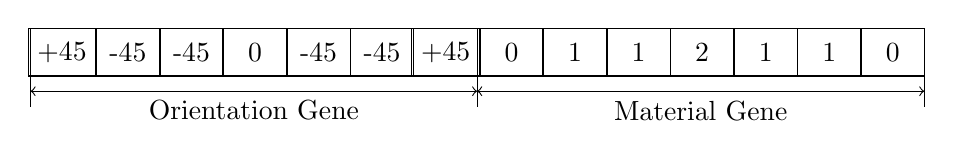
\begin{tikzpicture}
\tikzstyle{rec} = [rectangle, minimum width=0.8cm,minimum height=0.6cm, text
centered, draw=black]
\node (gene11) [rec] {+45};
\node (gene2) [rec] at ($(gene11.east)+(0.4cm,0)$)  {-45};
\node (gene3) [rec] at ($(gene2.east)+(0.4cm,0)$)  {-45};
\node (gene4) [rec] at ($(gene3.east)+(0.4cm,0)$)  {0};
\node (gene5) [rec] at ($(gene4.east)+(0.4cm,0)$)  {-45};
\node (gene6) [rec] at ($(gene5.east)+(0.4cm,0)$)  {-45};
\node (last) [rec] at ($(gene6.east)+(0.4cm,0)$)  {+45};
\node (gene1) [rec] at ($(last.east)+(0.4cm,0)$){0};
\node (gene2) [rec] at ($(gene1.east)+(0.4cm,0)$)  {1};
\node (gene3) [rec] at ($(gene2.east)+(0.4cm,0)$)  {1};
\node (gene4) [rec] at ($(gene3.east)+(0.4cm,0)$)  {2};
\node (gene5) [rec] at ($(gene4.east)+(0.4cm,0)$)  {1};
\node (gene6) [rec] at ($(gene5.east)+(0.4cm,0)$)  {1};
\node (gene7) [rec] at ($(gene6.east)+(0.4cm,0)$)  {0};

\draw[-] ($(gene11.north)+(-0.4cm,0)$) -- ++(0, -1cm) coordinate (A);
\draw[-] ($(last.north)+(0.4cm,0)$) -- ++(0, -1cm) coordinate (B);
\draw[-] ($(gene7.north)+(0.4cm,0)$) -- ++(0, -1cm) coordinate (C);
\draw[<->] ($(A) + (0, 0.2cm)$) -- ($(B) + (0,0.2cm)$) node[pos=0.5,auto=right] {Orientation Gene};
\draw[<->] ($(B) + (0, 0.2cm)$) -- ($(C) + (0,0.2cm)$) node[pos=0.5,auto=right] {Material Gene};

\end{tikzpicture}
\captionof{figure}{Parent 1 }
\label{fig:parent1}
\end{center}


\begin{center}
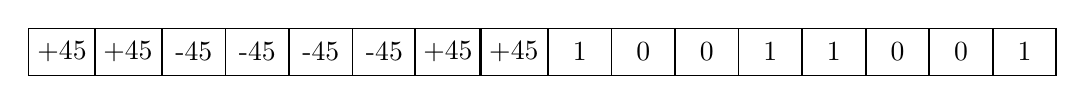
\begin{tikzpicture}
\tikzstyle{rec} = [rectangle, minimum width=0.8cm,minimum height=0.6cm, text
centered, draw=black]
\node (gene1) [rec] {+45};
\node (gene2) [rec] at ($(gene1.east)+(0.4cm,0)$)  {+45};
\node (gene3) [rec] at ($(gene2.east)+(0.4cm,0)$)  {-45};
\node (gene4) [rec] at ($(gene3.east)+(0.4cm,0)$)  {-45};
\node (gene5) [rec] at ($(gene4.east)+(0.4cm,0)$)  {-45};
\node (gene6) [rec] at ($(gene5.east)+(0.4cm,0)$)  {-45};
\node (gene7) [rec] at ($(gene6.east)+(0.4cm,0)$)  {+45};
\node (last) [rec] at ($(gene7.east)+(0.4cm,0)$)  {+45};
\node (gene1) [rec] at ($(last.east)+(0.4cm,0)$){1};
\node (gene2) [rec] at ($(gene1.east)+(0.4cm,0)$)  {0};
\node (gene3) [rec] at ($(gene2.east)+(0.4cm,0)$)  {0};
\node (gene4) [rec] at ($(gene3.east)+(0.4cm,0)$)  {1};
\node (gene5) [rec] at ($(gene4.east)+(0.4cm,0)$)  {1};
\node (gene6) [rec] at ($(gene5.east)+(0.4cm,0)$)  {0};
\node (gene7) [rec] at ($(gene6.east)+(0.4cm,0)$)  {0};
\node (gene7) [rec] at ($(gene7.east)+(0.4cm,0)$)  {1};
\end{tikzpicture}
\captionof{figure}{Parent 2 }
\label{fig:parent2}
\end{center}

\begin{center}
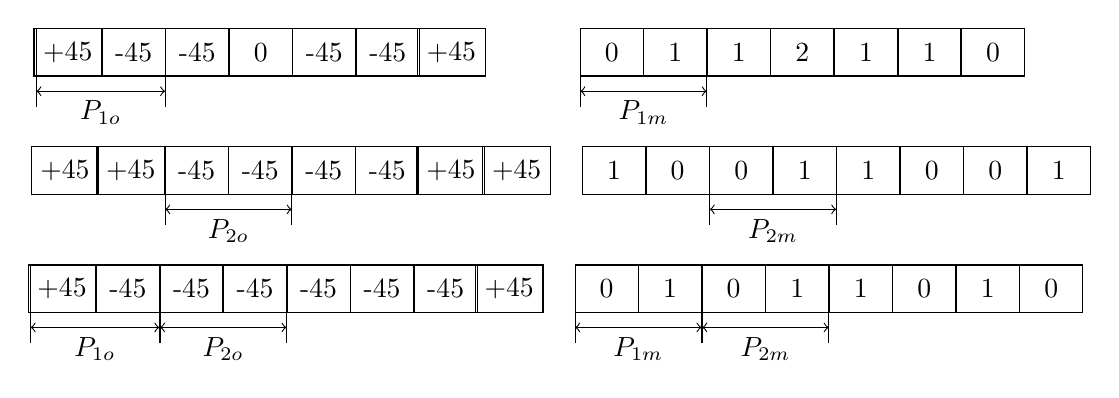
\begin{tikzpicture}
\tikzstyle{rec} = [rectangle, minimum width=0.8cm,minimum height=0.6cm, text
centered, draw=black]
\node (gene11) [rec] {+45};
\node (gene2) [rec] at ($(gene11.east)+(0.4cm,0)$)  {-45};
\node (gene3) [rec] at ($(gene2.east)+(0.4cm,0)$)  {-45};
\node (gene4) [rec] at ($(gene3.east)+(0.4cm,0)$)  {0};
\node (gene5) [rec] at ($(gene4.east)+(0.4cm,0)$)  {-45};
\node (gene6) [rec] at ($(gene5.east)+(0.4cm,0)$)  {-45};
\node (last) [rec] at ($(gene6.east)+(0.4cm,0)$)  {+45};

\draw[-] ($(gene11.north)+(-0.4cm,0)$) -- ++(0, -1cm) coordinate (A);
\draw[-] ($(gene2.north)+(0.4cm,0)$) -- ++(0, -1cm) coordinate (B);
\draw[<->] ($(A) + (0, 0.2cm)$) -- ($(B) + (0,0.2cm)$) node[pos=0.5,auto=right] {$P_{1o}$};
\node (gene1) [rec] at ($(last.east)+(1.6cm,0)$){0};
\node (gene2) [rec] at ($(gene1.east)+(0.4cm,0)$)  {1};
\node (gene3) [rec] at ($(gene2.east)+(0.4cm,0)$)  {1};
\node (gene4) [rec] at ($(gene3.east)+(0.4cm,0)$)  {2};
\node (gene5) [rec] at ($(gene4.east)+(0.4cm,0)$)  {1};
\node (gene6) [rec] at ($(gene5.east)+(0.4cm,0)$)  {1};
\node (gene7) [rec] at ($(gene6.east)+(0.4cm,0)$)  {0};
\draw[-] ($(gene1.north)+(-0.4cm,0)$) -- ++(0, -1cm) coordinate (A);
\draw[-] ($(gene2.north)+(0.4cm,0)$) -- ++(0, -1cm) coordinate (B);
\draw[<->] ($(A) + (0, 0.2cm)$) -- ($(B) + (0,0.2cm)$) node[pos=0.5,auto=right] {$P_{1m}$};

% parent2 

\node (genep2) [rec] at ($(gene11.west)+(0.4cm,-1.5cm)$) {+45};
\node (gene2) [rec] at ($(genep2.east)+(0.4cm,0)$)  {+45};
\node (gene3) [rec] at ($(gene2.east)+(0.4cm,0)$)  {-45};
\node (gene4) [rec] at ($(gene3.east)+(0.4cm,0)$)  {-45};
\node (gene5) [rec] at ($(gene4.east)+(0.4cm,0)$)  {-45};
\node (gene6) [rec] at ($(gene5.east)+(0.4cm,0)$)  {-45};
\node (gene7) [rec] at ($(gene6.east)+(0.4cm,0)$)  {+45};
\node (last) [rec] at ($(gene7.east)+(0.4cm,0)$)  {+45};
\draw[-] ($(gene3.north)+(-0.4cm,0)$) -- ++(0, -1cm) coordinate (A);
\draw[-] ($(gene4.north)+(0.4cm,0)$) -- ++(0, -1cm) coordinate (B);
\draw[<->] ($(A) + (0, 0.2cm)$) -- ($(B) + (0,0.2cm)$) node[pos=0.5,auto=right] {$P_{2o}$};
\node (gene1) [rec] at ($(last.east)+(0.8cm,0)$){1};
\node (gene2) [rec] at ($(gene1.east)+(0.4cm,0)$)  {0};
\node (gene3) [rec] at ($(gene2.east)+(0.4cm,0)$)  {0};
\node (gene4) [rec] at ($(gene3.east)+(0.4cm,0)$)  {1};
\node (gene5) [rec] at ($(gene4.east)+(0.4cm,0)$)  {1};
\node (gene6) [rec] at ($(gene5.east)+(0.4cm,0)$)  {0};
\node (gene7) [rec] at ($(gene6.east)+(0.4cm,0)$)  {0};
\node (gene7) [rec] at ($(gene7.east)+(0.4cm,0)$)  {1};
\draw[-] ($(gene3.north)+(-0.4cm,0)$) -- ++(0, -1cm) coordinate (A);
\draw[-] ($(gene4.north)+(0.4cm,0)$) -- ++(0, -1cm) coordinate (B);
\draw[<->] ($(A) + (0, 0.2cm)$) -- ($(B) + (0,0.2cm)$) node[pos=0.5,auto=right] {$P_{2m}$};

% offspring

\node (gene1) [rec] at ($(genep2.west)+(0.4cm,-1.5cm)$) {+45};
\node (gene2) [rec] at ($(gene1.east)+(0.4cm,0)$)  {-45};
\node (gene3) [rec] at ($(gene2.east)+(0.4cm,0)$)  {-45};
\node (gene4) [rec] at ($(gene3.east)+(0.4cm,0)$)  {-45};
\node (gene5) [rec] at ($(gene4.east)+(0.4cm,0)$)  {-45};
\node (gene6) [rec] at ($(gene5.east)+(0.4cm,0)$)  {-45};
\node (gene7) [rec] at ($(gene6.east)+(0.4cm,0)$)  {-45};
\node (last) [rec] at ($(gene7.east)+(0.4cm,0)$)  {+45};

\draw[-] ($(gene1.north)+(-0.4cm,0)$) -- ++(0, -1cm) coordinate (A);
\draw[-] ($(gene2.north)+(0.4cm,0)$) -- ++(0, -1cm) coordinate (B);
\draw[<->] ($(A) + (0, 0.2cm)$) -- ($(B) + (0,0.2cm)$) node[pos=0.5,auto=right] {$P_{1o}$};

\draw[-] ($(gene3.north)+(-0.4cm,0)$) -- ++(0, -1cm) coordinate (A);
\draw[-] ($(gene4.north)+(0.4cm,0)$) -- ++(0, -1cm) coordinate (B);
\draw[<->] ($(A) + (0, 0.2cm)$) -- ($(B) + (0,0.2cm)$) node[pos=0.5,auto=right] {$P_{2o}$};

\node (gene1) [rec] at ($(last.east)+(0.8cm,0)$){0};
\node (gene2) [rec] at ($(gene1.east)+(0.4cm,0)$)  {1};
\node (gene3) [rec] at ($(gene2.east)+(0.4cm,0)$)  {0};
\node (gene4) [rec] at ($(gene3.east)+(0.4cm,0)$)  {1};
\node (gene5) [rec] at ($(gene4.east)+(0.4cm,0)$)  {1};
\node (gene6) [rec] at ($(gene5.east)+(0.4cm,0)$)  {0};
\node (gene7) [rec] at ($(gene6.east)+(0.4cm,0)$)  {1};
\node (gene7) [rec] at ($(gene7.east)+(0.4cm,0)$)  {0};

\draw[-] ($(gene1.north)+(-0.4cm,0)$) -- ++(0, -1cm) coordinate (A);
\draw[-] ($(gene2.north)+(0.4cm,0)$) -- ++(0, -1cm) coordinate (B);
\draw[<->] ($(A) + (0, 0.2cm)$) -- ($(B) + (0,0.2cm)$) node[pos=0.5,auto=right] {$P_{1m}$};
\draw[-] ($(gene3.north)+(-0.4cm,0)$) -- ++(0, -1cm) coordinate (A);
\draw[-] ($(gene4.north)+(0.4cm,0)$) -- ++(0, -1cm) coordinate (B);
\draw[<->] ($(A) + (0, 0.2cm)$) -- ($(B) + (0,0.2cm)$) node[pos=0.5,auto=right] {$P_{2m}$};

\end{tikzpicture}
\captionof{figure}{Crossover Operation}
\label{fig:parent1}
\end{center}

\begin{center}
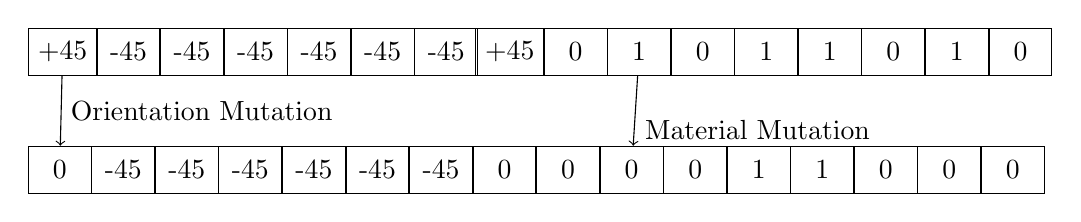
\begin{tikzpicture}
\tikzstyle{rec} = [rectangle, minimum width=0.8cm,minimum height=0.6cm, text
centered, draw=black]
\node (gene11) [rec] {+45};
\node (gene2) [rec] at ($(gene11.east)+(0.4cm,0)$)  {-45};
\node (gene3) [rec] at ($(gene2.east)+(0.4cm,0)$)  {-45};
\node (gene4) [rec] at ($(gene3.east)+(0.4cm,0)$)  {-45};
\node (gene5) [rec] at ($(gene4.east)+(0.4cm,0)$)  {-45};
\node (gene6) [rec] at ($(gene5.east)+(0.4cm,0)$)  {-45};
\node (gene7) [rec] at ($(gene6.east)+(0.4cm,0)$)  {-45};
\node (last) [rec] at ($(gene7.east)+(0.4cm,0)$)  {+45};
\node (gene1) [rec] at ($(last.east)+(0.4cm,0)$){0};
\node (gene2u) [rec] at ($(gene1.east)+(0.4cm,0)$)  {1};
\node (gene3) [rec] at ($(gene2u.east)+(0.4cm,0)$)  {0};
\node (gene4) [rec] at ($(gene3.east)+(0.4cm,0)$)  {1};
\node (gene5) [rec] at ($(gene4.east)+(0.4cm,0)$)  {1};
\node (gene6) [rec] at ($(gene5.east)+(0.4cm,0)$)  {0};
\node (gene7) [rec] at ($(gene6.east)+(0.4cm,0)$)  {1};
\node (gene7) [rec] at ($(gene7.east)+(0.4cm,0)$)  {0};

\node (gene12) [rec] at ($(gene11.west)+(0.4cm,-1.5cm)$) {0};
\node (gene2) [rec] at ($(gene12.east)+(0.4cm,0)$)  {-45};
\node (gene3) [rec] at ($(gene2.east)+(0.4cm,0)$)  {-45};
\node (gene4) [rec] at ($(gene3.east)+(0.4cm,0)$)  {-45};
\node (gene5) [rec] at ($(gene4.east)+(0.4cm,0)$)  {-45};
\node (gene6) [rec] at ($(gene5.east)+(0.4cm,0)$)  {-45};
\node (gene7) [rec] at ($(gene6.east)+(0.4cm,0)$)  {-45};
\node (last) [rec] at ($(gene7.east)+(0.4cm,0)$)  {0};
\node (gene1) [rec] at ($(last.east)+(0.4cm,0)$)  {0};
\node (gene2d) [rec] at ($(gene1.east)+(0.4cm,0)$)  {0};
\node (gene3) [rec] at ($(gene2d.east)+(0.4cm,0)$)  {0};
\node (gene4) [rec] at ($(gene3.east)+(0.4cm,0)$)  {1};
\node (gene5) [rec] at ($(gene4.east)+(0.4cm,0)$)  {1};
\node (gene6) [rec] at ($(gene5.east)+(0.4cm,0)$)  {0};
\node (gene7) [rec] at ($(gene6.east)+(0.4cm,0)$)  {0};
\node (gene7) [rec] at ($(gene7.east)+(0.4cm,0)$)  {0};

\draw[->] (gene11) -- (gene12) node[pos=0.5,auto=left] {Orientation Mutation};
\draw[->] (gene2u) -- (gene2d) node[pos=0.5,auto=left] {Material Mutation};
\end{tikzpicture}
\captionof{figure}{Mutation}
\label{fig:muation}
\end{center}



\subsection{Design Problem I}


The aim is to minimize the mass of a composite laminate for a targeted strength
ratio by Tsai-wu failure theory. The design variable are the ply angles and the
number of layers.

Find: $\{\theta_k, n\}$ $\theta_k \in \{ 0,\text{+}45,\text{-}45,90\}$ 

Minimize: weight

Subject to: safety factor and first ply failure constraint


\subsection{Design Problem II}
The aim is to mimimize the combined cost and weight of hybrid composite
laminate under various loading cases, so the design variable not only include
the ply angles and number of layers, but also the material of each lamina. 


Find: $\{\theta_k,\text{mat}_k, n\}$ $\theta_k \in \{ 0,\text{+}45,\text{-}45,90\}$ $\text{mat}_k \in \{CA, GR, GL \}$

Minimize: 
\begin{equation}
	F=\frac{\text { Cost }}{C_{\text {min }}}+\frac{\text { Weight }}{W_{\text {min }}}
\end{equation}

Subject to: safety factor and first ply failure constraint


Here CA, GF, and GL represent carbon/epoxy, graphite/epoxy, and glass/epoxy,
and each CA, GF, and GL layer is assumed to cost 8, 2.5 and 1 monetary units,
respectively. $C_{\text{min}}$ and $W_{\text{min}}$ represent the cost and
weight corresponding to the laminates with minimum cost and minimum weight
obtained from previous problem.








\section{Numberical results and Discussion}
The numberical results were obtained for a carbon/epoxy, graphite/epoxy and
glass/epoxy, respectively, the material properties as shown in Table
\ref{tab:mat}. The thickness of the each lamina is 0.165mm.

\captionof{table}{Comparsion of carbon/epoxy, graphite/epoxy, and glass/epoxy properties}
\begin{tabular}{cccccc}
	\toprule
	Property								   & Symbol				  & Unit  &  Carbon/Epoxy&  Graphite/Epoxy  &  Glass/Epoxy   \\
	\midrule																								  
	Longitudinal elastic modulus			   & $E_1$				  & GPa   &  116.6       &  181             &  38.6           \\
	Traverse elastic modulus				   & $E_2$				  & GPa   &  7.67        &  10.3            &  8.27           \\
	Major Poisson's ratio					   & $v_{12}$			  &       &  0.27        &  0.28            &  0.26           \\
	Shear modulus							   & $G_{12}$			  & GPa   &  4.17        &  7.17            &  4.14           \\
	Ultimate longitudinal tensile strength     & $(\sigma_1^T)_{ult}$ & MP    &  2062        &  1500            &  1062            \\
	Ultimate longitudinal compressive strength & $(\sigma_1^C)_{ult}$ & MP    &  1701        &  1500            &  610             \\
	Ultimate transverse tensile strength       & $(\sigma_2^T)_{ult}$ & MPa   &  70          &  40              &  31              \\
	Ultimate transverse compressive strength   & $(\sigma_2^C)_{ult}$ & MPa   &  240         &  246             &  118              \\
	Ultimate in-plane shear strength           & $(\tau_{12})_{ult}$  & MPa   &  105         &  68              &  72               \\
	Density                                    & $\rho$               & $g/cm^3$ &  1.605    &  1.590           &  1.903               \\
	Cost                                       &                      &       &  8           &  2.5             &  1               \\
	\bottomrule
\end{tabular}
\label{tab:mat}


\captionof{table}{Comparative study of different composite materials for a defined strength ratio}

\begin{tabular}{ccccccc}
	\toprule
	Load         &  Problem             & Stacking sequence        & Strength ratio  & Mass &  Cost   & Layer    \\
	\midrule
	  \multirow{4}{*}{$N_{x}=1e6$ N}  &    I      &  $[0_{cr6}]$                             & 2.041           & 0.318 &  48.0  & 6  \\
									  &     I     &  $[0_{gr9}]$                      & 2.227           & 0.472 &  22.5  & 9  \\
		         	                  &     I     &  $[0_{gl12}]$                             & 2.103           & 0.753 &  12.0  & 12  \\
									  &     II    &  $[0_{gr4}/0_{gl}/0_{gr4}]$                      & 2.031           & 0.482 &  21.0  & 9 \\
	\bottomrule
\end{tabular}


\begin{tabular}{ccccccc}
	\toprule
	Load                             &Problem & Stacking sequence        & Strength ratio  & Mass &  Cost   & Layer    \\
	\midrule
	 \multirow{4}{*}{$N_{y}=1e6$ N}  &  I        &  $[90_{cr6}]$                             & 2.041           & 0.318 &  48.0  & 6  \\
					                 &  I        &  $[90_{gr9}]$                      & 2.227           & 0.472 &  22.5  & 9  \\
           		 	                 &  I        &  $[90_{gl12}]$                             & 2.103           & 0.753 &  12.0  & 12  \\
									 &  II       &  $[90_{gr4}/90_{gl}/90_{gr4}]$                      & 2.031           & 0.482 &  21.0  & 9 \\
	\bottomrule
\end{tabular}


\begin{tabular}{ccccccc}
	\toprule
	Load                               &Problem   & Stacking sequence        & Strength ratio  & Mass &  Cost   & Layer    \\
	\midrule
	\multirow{4}{*}{$N_{xy}=1e6$ N}	   &    I      &  $[\text{-}45_{cr6}/\text{+}45_{cr14}/\text{-}45_{cr6}]$                  & 2.013           & 1.377 &  208.0  & 26  \\
									   &    I      &  $[\text{-}45_{gr5}/\text{+}45_{gr23}/\text{-}45_{gr5}]$                & 2.105           & 1.732 &  82.5   & 33  \\
									   &    I      &  $[\text{-}45_{gl17}/\text{+}45_{gl76}/\text{-}45_{gl17}]$               & 2.011           & 6.908 &  110.0  & 110  \\
									   &    II     &  $[\text{-}45_{ca3}/\text{+}45_{ca4}/\text{+}45_{gr6}/\text{+}45_{ca}]_s$    & 2.074    & 1.424 &  150    & 27 \\
	\bottomrule
\end{tabular}

\begin{tabular}{ccccccc}
	\toprule
	Load                                                        &Problem& Stacking sequence                                & Strength ratio  & Mass &  Cost   & Layer    \\
	\midrule
	\multirow{3}{*}{\makecell{$N_x=1e6$ N\\ $N_y=1e6$ N}}       &       I                &  $[\text{-}45_{cr6}/\text{+}45_{cr6}]_s$                        & 2.026           & 1.271 &  192.0  & 24  \\
																&       I                &  $[\text{+}45_{gr10}/\text{-}45_{gr21}/\text{+}45_{gr10}]$            & 2.024           & 2.151 &  102.5  & 41  \\
																&       I                &  $[\text{-}45_{gl35}/\text{+}45_{gl_73}/\text{+}45_{gl35}]$            & 2.001           & 8.980 &  143.0  & 143  \\
																&       II                &
	$[\text{-}45_{gr9}/\text{+}45_{gr_9}/\text{-}45_{ca2}/\text{+}45_{ca2}]_s$            & 2.054         & 2.313 &
																		  154& 44  \\
	\bottomrule
\end{tabular}

\begin{tabular}{ccccccc}
	\toprule
	Load                                                    &   Problem          & Stacking sequence                          & Strength ratio  & Mass &  Cost   & Layer    \\
	\midrule
	\multirow{4}{*}{\makecell{$N_{x}=1e6$ N \\ $N_{y}=1e6$ N  \\ $N_{xy}=1e6$} }  &      I   &  $[\text{+}45_{cr12}]$                            & 2.041           & 0.636 &  96.0  & 12  \\
													    						  &      I   &  $[\text{+}45_{gr18}]$                            & 2.227           & 0.945 &  45.0  & 45  \\
			 &  I                  &  $[\text{+}45_{gl23}]$                            & 2.015           & 1.444 &  23.0  & 23  \\
			 &  II                 &  $[\text{+}45_{gl}/\text{+}45_{gr16}/\text{+}45_{gr}]$          & 2.031           & 0.965 &  42.0  & 18 \\
	\bottomrule
\end{tabular}




\section{Conclusions}
In this paper, a combination of CLT and GA is employed to minimize the weight
and cost of a single-material and hybrid composite laminate, respectively,
under various in-plane loading cases. GA is proposed to obtain the global
optimum design, results are presented in two sections, stacking sequence
optimization for a single material laminate, and combined weight and cost
optimization of a carbon/epoxy, graphite/epoxy, and glass/epoxy hybrid
laminate.

\section{Acknowledgements}
This is work was supported by 


%\end{multicols}
%\end{multicols}


\bibliographystyle{plain}
\bibliography{laminate_design}


\end{document}


\begin{comment}
\begin{center}
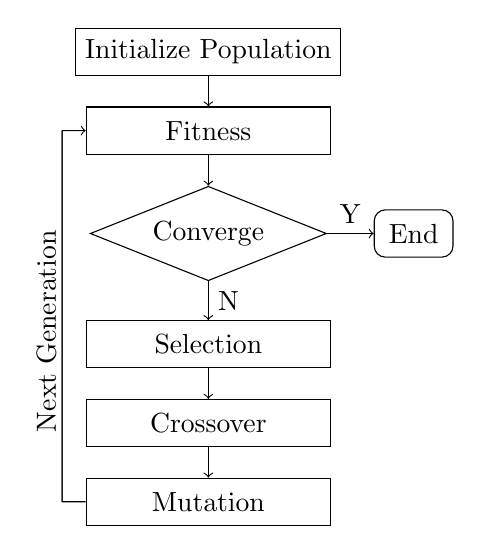
\begin{tikzpicture}
\tikzstyle{startstop} = [rectangle, rounded corners, minimum width=1.0cm,minimum height=0.6cm, 
                        text centered, draw=black]
\tikzstyle{io} = [trapezium, trapezium left angle=70, trapezium right angle=110, minimum width=2cm, 
                 minimum height=0.6cm, text centered, draw=black]
\tikzstyle{process} = [rectangle, minimum width=3.1cm, minimum height=0.6cm, text centered, draw=black]
\tikzstyle{decision} = [diamond,minimum width=3cm, minimum height=1.2cm, draw=black]
\node (population) [process] {Initialize Population};
\node (fitness) [process, below of=population] {Fitness};
\node (decision) [decision] at ($(fitness.south)+(0,-1.0cm)$) {} node at (decision.base) {Converge};
\node (share-fitness) at ($(decision.south)+(0,-0.8cm)$) [process] {Selection};
\node (selection) [process,below of=share-fitness] {Crossover};
\node (crossover) [process,below of=selection]  {Mutation};
\node (end) [startstop] at ($(decision.east)+(1.1cm,0)$)  {End};
\draw [->] (population) -- (fitness);
\draw [->] (fitness) -- (decision);
\draw [->] (decision) -- (share-fitness) node[auto=left,pos=0.5]{N};
\draw [->] (share-fitness.south) -- (selection.north) ;
\draw [->] (selection.south) -- (crossover.north);
\draw [->] (decision.east) -- (end.west) node[auto=left,pos=0.5]{Y};

% draw intersection
\draw [white] (fitness.west) -- ++(-0.5cm,0) coordinate (A);
\draw [white] (crossover.west) -- ++(-0.3cm,0) coordinate (B)-- ++(0,6cm) coordinate (C) ; 
\draw (crossover.west) -- ++(-0.3cm,0) -- (intersection cs: first line={(fitness.west)--(A)}, 
      second line={(B)--(C)}) coordinate (D);
\draw (B) -- (D) node[auto=left,pos=0.8,rotate=90,xshift=-0.2cm,yshift=0.2cm] {Next Generation} ;
\draw [<-] (fitness.west) -- (D);
\end{tikzpicture}
\captionof{figure}{GA Procedure with Share Function}
\label{plot:GA}
\end{center}
\end{comment}

